\documentclass[a4paper,12pt]{report}
\usepackage[utf8]{inputenc}


\usepackage{tikz}
\usetikzlibrary{calc}
\usepackage{subcaption}

\begin{document}

\thispagestyle{empty}

\begin{figure}[h!]
    \centering
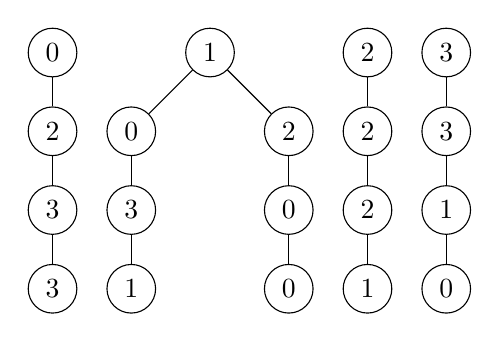
\begin{tikzpicture}
    \node[shape=circle,draw=black] (0) at (0,0) {0};
    \node[shape=circle,draw=black] (4) at (0,-1) {2};
    \node[shape=circle,draw=black] (5) at (0,-2) {3};
    \node[shape=circle,draw=black] (6) at (0,-3) {3};
    
    \node[shape=circle,draw=black] (1) at (2,0) {1};
    \node[shape=circle,draw=black] (7) at (1,-1) {0};
    \node[shape=circle,draw=black] (8) at (1,-2) {3};
    \node[shape=circle,draw=black] (9) at (1,-3) {1};
    
    \node[shape=circle,draw=black] (10) at (3,-1) {2};
    \node[shape=circle,draw=black] (11) at (3,-2) {0};
    \node[shape=circle,draw=black] (12) at (3,-3) {0};
    
    
    \node[shape=circle,draw=black] (2) at (4,0) {2};
    \node[shape=circle,draw=black] (13) at (4,-1) {2};
    \node[shape=circle,draw=black] (14) at (4,-2) {2};
    \node[shape=circle,draw=black] (15) at (4,-3) {1};
    
    \node[shape=circle,draw=black] (3) at (5,0) {3};
    \node[shape=circle,draw=black] (16) at (5,-1) {3};
    \node[shape=circle,draw=black] (17) at (5,-2) {1};
    \node[shape=circle,draw=black] (18) at (5,-3) {0};

    \path [-] (0) edge node {} (4);
    \path [-] (4) edge node {} (5);
    \path [-] (5) edge node {} (6);
    
    \path [-] (1) edge node {} (7);
    \path [-] (7) edge node {} (8);
    \path [-] (8) edge node {} (9);
    
    \path [-] (1) edge node {} (10);
    \path [-] (10) edge node {} (11);
    \path [-] (11) edge node {} (12);
    
    \path [-] (2) edge node {} (13);
    \path [-] (13) edge node {} (14);
    \path [-] (14) edge node {} (15);
    
    \path [-] (3) edge node {} (16);
    \path [-] (16) edge node {} (17);
    \path [-] (17) edge node {} (18);
\end{tikzpicture}
\caption{Example of one of the worst-case scenarios with parameters $K=5$ and $b=4$}
    \label{tree:2}
\end{figure}
\end{document}
